
\subsection{Analytical comparison of methods}

Both the direct method of section~\ref{sec:grad} and the EM algorithm of section~\ref{sec:EM_SSM}
have their strengths and weaknesses. Neither of them can be said to eclipse the other in an absolute sense.
In this section we will go through some features of the said algorithms found in the literature.
Then a more detailed analysis will be performed on two essential aspects of any estimation algorithm:
the convergence properties, i.e. when should one expect the algorithm to find a local maximum and
the computational requirements of the algorithms.

\textcite{Cappe2005} contains a list of arguments in favor of either of the methods. The following list includes
those and additional points with comments:
\begin{description}
  \item[Direct]\hfill
\begin{itemize}
  \item\emph{No smoother needed} The log-likelihood, or an approximation to it, can be evaluated
  with forward-filtering
  \item\emph{No M-step}. There is no need to figure out model-dependent maximization
  formulas even in nonlinear models 
  \item\emph{Faster convergence}. Advanced gradient-based optimization
  methods can reach convergence speeds that are close to quadratic
\end{itemize}
  \item[EM]\hfill
  \begin{itemize}
  \item \emph{Simple to implement}. This argument is often put forward in favor of the EM
 algorithm. However in practice when using the gradient-based method one would use any one of
the off-the-self nonlinear optimizers and not re-implement one. Thus which one is easier to implement
boils down to gradient computation. If the model is linear or linear-in-the-parameters the EM
algorithm doesn't need any gradient information.
  \item\emph{Parameter constraints}. In \textcite{Cappe2005} it is argued that
since the M-step maximization equations are so simple, including parameter constraints
are easier in the EM algorithm. This again depends on if the model is linear or linear-in-the-parameters.
  \item\emph{Parameterization independent}. This again depends on if one has to use gradient-based
 optimization in the M-step. If not, then the EM algorithm is parameterization independent. In the gradient-based
 method the gradient and the Hessian, and so the convergence, are affected by the parameterization.
\end{itemize} 
\end{description}

\clearpage
%%%%%%%%%%%%%%%%%%%%%%%%%%%%%%%%%%%%%%%%%%%%%%%%%%%%%%%%%
%%%% BALLISTIC OBJECT %%%%%%%%%%%%%%%%%%%%%%%%%%%%%%%%%%%
%%%%%%%%%%%%%%%%%%%%%%%%%%%%%%%%%%%%%%%%%%%%%%%%%%%%%%%%%

\subsection{Endoathmospheric flight of a ballistic projectile}\label{sec:ballistic}
Let us consider a situation where a ballistic projectile is launched
from the ground into the air. We assume that the situation is governed by Newtonian
mechanics and that the projectile experiences a constant known gravitational
force, directed towards the ground. In addition we assume a \emph{constant}
drag force directed orthogonally to the gravitational force. This is clearly
an oversimplification, since in a more realistic model the drag
force is proportional to velocity and directed against it. Furthermore
the drag force is higly dependent on air density and so the altitide. \parencite{ristic2004beyond}.
Nevertheless, we make the aforementioned simplification to keep to resulting
SSM linear. The modelling error is mitigated slightly by introducing
additive white noise to both forces.

We obtain a sequence of range measurements with a radar,
so that our data consists of the noisy two dimensional locations 
of the object as measured at time points $\brac{t_k}_{k=1}^T$.
We assume a constant interval $\tau$ between the time points. With these 
considerations, the system can be cast into a linear-Gaussian SSM. 

In continous time and for a single coordinate $\chi$, 
the dynamics can now be written as
\begin{align}
	\dod{}{t}\bm{\chi(t) \\ \dot{\chi}(t) } &= 
	\bm{0 & 1\\0 & 0}\bm{\chi(t) \\ \dot{\chi}(t) } + \bm{0\\1}g_\chi + \bm{0\\1}\beta(t),
	\label{eq:ct_linear}
\end{align}
where $g_\chi<0$ is the mean of the force and $\beta(t)$ can be considered
a white noise process with variance (or spectral density) $q_\chi$. 
The state then contains the position and its first time derivative, i.e the velocity. 

% with
% \begin{align}
% 	\x(t) &= \bm{x(t) & \dot{x}(t) & \ddot{x}(t) & y(t) & \dot{y}(t) & \ddot{y}(t)}^\tr\\
% 	\v{F}&=\bm{
% 	&&1&&&\\
% 	&&&1&&\\
% 	&&&&1&\\
% 	&&&&&1\\
% 	&&&&&\\
% 	&&&&&\\
% 	}
% 	\label{tablelabel}
% \end{align}

To discretize the dynamics, we will apply a simple integration scheme where 
$\x(t)=\x(t_k)$ when $t\in\big[t_k,t_{k+1}\big)$ \parencite{bar2004estimation}.
The system will be modeled in two dimensional Cartesian coordinates so that $d_x=4$, i.e
two components for position and two for velocity. The state at time $k$ is then
\begin{align}
	\xk &=
	\bm{\chi_k & \dot{\chi}_k  
	  & \gamma_k & \dot{\gamma}_k }^\tr
	\label{eq:ballistic2D_state}
\end{align}
where $\dot{\chi}_k = \eval{\dod{\chi(t)}{t}}_{t=t_k}$ and analogously for $\dot{\gamma}_k$.
The corresponding measurement without the additive noise is
\begin{align}
	\yk-\v{r}_k &= \bm{\chi_k & \gamma_k }^\tr.
	\label{eq:ballistic2D_measurementsl}
\end{align}


\noindent The discrete time linear-Gaussian SSM can now be written as
\begin{align}
	\begin{aligned}
	\x_k &= \v{A}\xkk+\v{u}+\q_{k-1},\qquad & 
	\q_{k-1} &\sim \N{\v{0}}{\v{Q}},\\
	\yk &= \v{H}\xk+\v{r}_k, & 					
	\v{r}_k 	&\sim \N{\v{0}}{\sigma_r^2\v{I}},
	\end{aligned}\label{eq:ballistic_model}
\end{align}
where
\begin{align*}
	\v{A}&=\bm{
	1& \tau & 	& 		\\
	 &	1	& 	&		\\
	 &		& 1	& \tau 	\\
	 &		&	& 1
	},
	&
	\v{u} &= \bm{0 \\ g_\chi \\ 0 \\ g_\gamma},\\
	%
	\v{Q}&=\bm{
	\sfrac{1}{3}\sigma_\chi^2\tau^3 & \sfrac{1}{2}\sigma_\chi^2\tau^2 & 	& 		\\
	\sfrac{1}{2}\sigma_\chi^2\tau^2 &	\sigma_\chi^2\tau & 	&		\\
	 &		& \sfrac{1}{3}\sigma_\gamma^2\tau^3	& \sfrac{1}{2}\sigma_\gamma^2\tau^2 	\\
	 &		&	\sfrac{1}{2}\sigma_\gamma^2\tau^2 & \sigma_\gamma^2\tau
	},
	&
	\v{H} &= \bm{1 & 0 & 0 & 0 \\ 0 & 0 & 1 & 0}.
\end{align*}
Additionally, the initial state $\x_0$ is assumed to be known
with $\x_0=\bm{0 & \cos(\alpha_0)v_0 & 0 & \sin(\alpha_0)v_0}^\tr$.

Figure~\ref{fig:ballistic2D_simulation} presents an example trajectory with
the hidden state components obtained by simulation and the correponding
simulated noisy measurements. The simulated model was the discretized
linear-Gaussian model in Equation~\eqref{eq:ballistic_model} with  
the parameter values presented in Table~\ref{table:ballistic_param}.

\begin{table}[htbp]
\caption{Parameter values used for simulation in Section~\ref{sec:ballistic}}
\label{table:ballistic_param}
\centering
\footnotesize
\begin{tabular}{>{$}c<{$}Ss@{\hspace{1.5cm}}>{$}c<{$}Ss}
\toprule
\multicolumn{1}{c}{Parameter}&%
\multicolumn{1}{c}{Value}&%
\multicolumn{1}{c@{\hspace{1.5cm}}}{Unit}&%
\multicolumn{1}{c}{Parameter}&%
\multicolumn{1}{c}{Value}&%
\multicolumn{1}{c}{Unit}\\
\midrule
	\sigma_\chi		&	1.2			&	m			&	\tau			&	0.01 		& s\\
	\sigma_\gamma 	&	0.8			&	m			&	\sigma_r		& 	2.5 		& m	\\	 	
 	g_\chi			&	-1.8		&	m/s^2		&	\alpha_0		& 	60 		& \degree\\	 	
	g_\gamma 		&	-9.81		&	m/s^2		&	v_0 			&	40	 	& m/s\\
\bottomrule	 	
\end{tabular}
\end{table}

Let us then proceed to estimating some of the parameters by using the noisy
measurements as input to the two parameter estimation methods we have been considering.
We choose parameters $\Th_{\mathrm{B}}=\brac{g_\chi,g_\gamma,\sigma_r}$, i.e. the
accelerations caused by the drag force and gravitation as well as the measurement noise
standard deviation. The true values, i.e. the values which were used for generating the
measurements are presented in Table~\ref{table:ballistic_param}. To inspect the effect of
the initial guess as well as well as that of the specific measurement dataset, we ran
$M=100$ simulations with the initial estimate for each parameter $\theta_i$ picked 
from the uniform distribution $U\brak{0,2\theta_i}$. The lengths of the simulated measurent
datasets were around $N\approx 1400$ with some variance caused by always stopping
the simulation when $\gamma_k<0$ for some $k$. For each simulated dataset and the associated
initial estimate we ran the EM and the BFGS parameter estimation methods for joint estimation
of the three parameters. The results are presented in Figure~\ref{fig:ballistic_est},
which contains eight separate panels: one per parameter and estimation method and
the likelihoods for both estimation methods. One line is plotted
in every panel for every simulated dataset and the panels display their quantities
as a function of the iteration number of the estimation method. Thus 
Figure~\ref{fig:ballistic_est} displays the convergence behaviour of the 
parameter estimation methods as a function of the initial estimate (for a limited
range of initial estimates). It is important to note that the iteration numbers are
not directly comparable between the parameter estimation methods so that one
shoudn't draw conclusions on the relative convergence rate betweeen the methods
based solely on Figure~\ref{fig:ballistic_est}.


\begin{figure}[htbp]%
    \centering%
    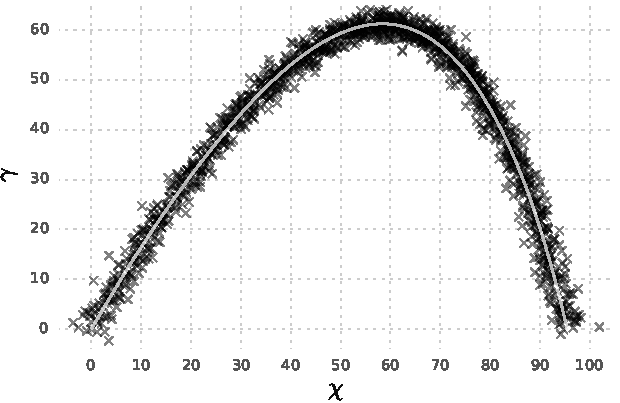
\includegraphics{img/ballistic_trajectory}%
	\caption{A simulation of the trajectory%
	%of the projectile in model~\eqref{eq:ballistic_model}.%
   	The measurements are denoted with crosses.}\label{fig:ballistic2D_simulation}
 \end{figure}

\begin{figure}[htb]%
    \centering%
	\makebox[\textwidth]{%
    \begin{subfigure}[t]{0.5\textwidth+0.4in}%
    	\caption{EM}\label{fig:ballistic_lh_em}%
    	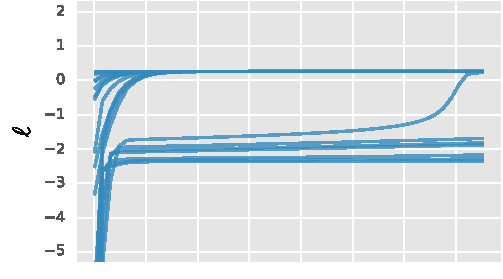
\includegraphics{img/ballistic_lh_em}%
    \end{subfigure}%
    \begin{subfigure}[t]{0.5\textwidth+0.4in}%
		\caption{BFGS}\label{fig:ballistic_lh_bf}%
		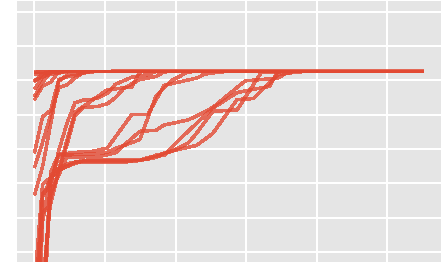
\includegraphics{img/ballistic_lh_bf}%
    \end{subfigure}}
    \caption{Convergence of the likelihood for $M=100$ simulated datasets
    with varying initial parameter estimates. 
    Both EM in \subref{fig:ballistic_lh_em} and BFGS
    in \subref{fig:ballistic_lh_bf} converge to the same
    likelihood value on this scale.}\label{fig:ballistic_lh}
\end{figure}
    

%\parencite{ristic2004beyond,Ratna2008,Lindsten2010}
 
 \begin{figure}[htb]%
    \centering%
    \makebox[\textwidth]{%
    \begin{subfigure}[t]{0.5\textwidth+0.4in}%
    	\caption{EM}
    	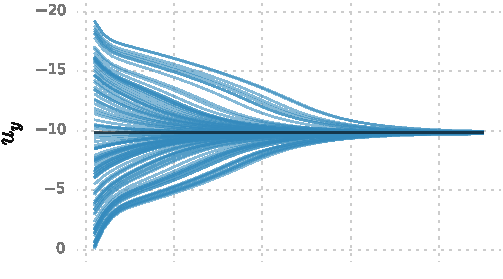
\includegraphics{img/ballistic_em_uy}%
    	%\caption{Convergence of the likelihood with EM}%
		%\label{fig:ballistic_lh_em}%
    \end{subfigure}%
    \begin{subfigure}[t]{0.5\textwidth+0.4in}%
		\caption{BFGS}
		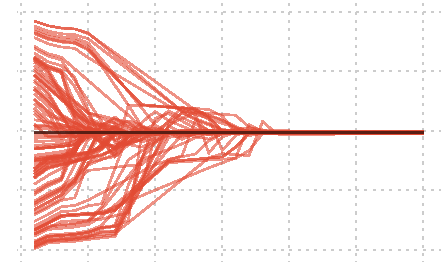
\includegraphics{img/ballistic_bf_uy}%
    	%\caption{Convergence of the likelihood with BFGS}%
		%\label{fig:ballistic_lh_bf}%
    \end{subfigure}}\\%
    \makebox[\textwidth]{%
    \begin{subfigure}[t]{0.5\textwidth+0.4in}%
    	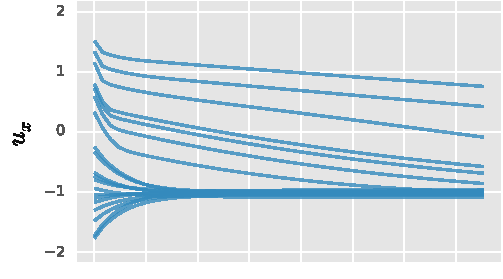
\includegraphics{img/ballistic_em_ux}%
    	%\caption{Convergence of the likelihood with EM}%
		%\label{fig:ballistic_lh_em}%
    \end{subfigure}%
    \begin{subfigure}[t]{0.5\textwidth+0.4in}%
		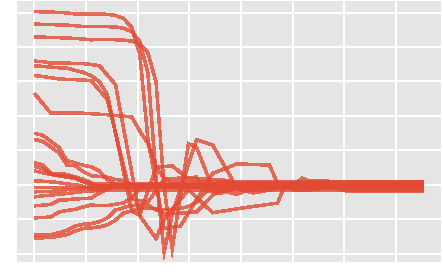
\includegraphics{img/ballistic_bf_ux}%
    	%\caption{Convergence of the likelihood with BFGS}%
		%\label{fig:ballistic_lh_bf}%
    \end{subfigure}}\\%
    \makebox[\textwidth]{%
	\begin{subfigure}[b]{0.5\textwidth+0.4in}%
    	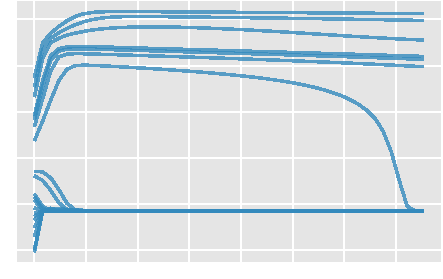
\includegraphics{img/ballistic_em_r}%
    	%\caption{Convergence of the likelihood with EM}%
		%\label{fig:ballistic_lh_em}%
    \end{subfigure}%
    \begin{subfigure}[b]{0.5\textwidth+0.4in}%
		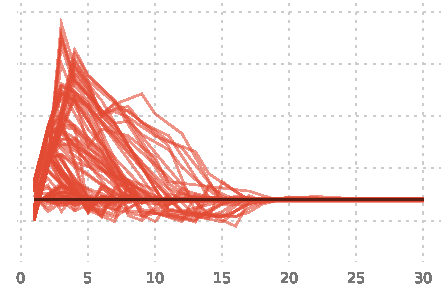
\includegraphics{img/ballistic_bf_r}%
    	%\caption{Convergence of the likelihood with BFGS}%
		%\label{fig:ballistic_lh_bf}%
    \end{subfigure}}%
    \caption{Convergence of the likelihood with EM and BFGS}\label{fig:ballistic_est}
 \end{figure}
 
\begin{table}[htbp]
	\caption{Estimated parameter values averaged over $100$ simulations in Section~\ref{sec:ballistic}}
	\label{table:ballistic_restults}
	\centering
	\sisetup{
		table-auto-round,
		table-format = 1.3
	}
	\footnotesize
	\begin{tabular}{rSSS}
\toprule
&\multicolumn{1}{c}{{\bfseries $g_\chi$}}&\multicolumn{1}{c}{{\bfseries $g_\gamma$}}&\multicolumn{1}{c}{{\bfseries $\sigma_r$}}\\\otoprule
True&-1.80000&-9.81000&1.50000\\
BFGS&-1.78372&-9.80360&1.49913\\
EM&-1.78372&-9.80473&1.49912\\
\bottomrule\end{tabular}

\end{table} 


\clearpage


%%%%%%%%%%%%%%%%%%%%%%%%%%%%%%%%%%%%%%%%%%%%%%%%%%%%%%%%%%%%%%%%
%%%%%%%%%%%%%%%%%%%% HEART %%%%%%%%%%%%%%%%%%%%%%%%%%%%%%%%%%%%%
%%%%%%%%%%%%%%%%%%%%%%%%%%%%%%%%%%%%%%%%%%%%%%%%%%%%%%%%%%%%%%%%

\subsection{Electrocardiograph analysis}

The second demonstration is concerned with a nonlinear model for
electrocardiograph (ECG) data, a short sequence of which is presented
in Figure~\ref{fig:ecg_data}. A realistic model for this data 
should take into account the quasi-periodic nature of ECG data,
i.e. the frequency must be allowed to vary with time.
Following the ideas in \textcite{Sarkka2012}, one possibility
is to write the model as a superposition of noisy resonators
with time-varying frequencies.

In continous time we can write a stochastic differential equation
for the $n$:th harmonic as
\begin{align}
	 \ddot{c}_n(t)&= -\omega(t)^2c_n(t)+\varepsilon_n(t),
	 %\dod[2]{c_n(t)}{t}
	\label{eq:noisy_resonator}
\end{align}
where $c_n(t)$ is the displacement from equilibrium at time $t$.
The angular velocity $\omega$ is related to the frequency $f$
by $\omega(t)=2\pi f(t)$ and  $\varepsilon_n(t)$ is additive
white noise with spectral density $q_n$. For constant frequency and
zero spectral density, the solution of Equation~\eqref{eq:noisy_resonator}
is well known to be $c_n(t)=\exp(i n \omega t+\phi_n)$, where $\phi_n\in\field{C}$ depends on 
the initial conditions.

Writing Equation~\eqref{eq:noisy_resonator} as a vector valued first order differential equation
and dividing the noise and the signal derivative by $n\omega(t)$, we get
\begin{align}
	\dod{}{t}\bm{c_n(t) \\ \widehat{\dot{c}}_n(t)} &= \bm{0 & \omega(t)^2 \\ -\omega(t) 0}\bm{c_n(t) \\
	\widehat{\dot{c}}_n(t)}+\bm{0\\1}
	\widehat{\varepsilon}_n(t).
	\label{eq:noisy_resonator_vec}
\end{align}
As explained in \textcite{Sarkka2012}, even if Equation~\eqref{eq:noisy_resonator_vec} is not an exact
representation of Equation~\eqref{eq:noisy_resonator}, its discretized version has more appealing
properties than that of the exact version. Furthermore, the process noise can account for some
modeling errors. 

Discretizing Equation~\eqref{eq:noisy_resonator_vec} at equispaced points $\brac{t_k}_{k=1}^T$
with interval $\tau$ and assuming $\omega(t)=\omega(t_k)\equiv \omega_k$ when $t\in\brak{t_k,t_{k+1}}$,
we get the following dynamic model for displacement $x^{(n)}$:
\begin{align}
	\bm{x_k^{(n)} \\ \dot{x}_k^{(n)}} &\sim 
	\N{\bm{\cos(n\omega_k) & \sin(n\omega_k) \\% 
	   -\sin(n\omega_k) & \cos(n\omega_k)}
	   \bm{x_{k-1}^{(n)} \\ \dot{x}_{k-1}^{(n)}}}
	  {\bm{0 & 0 \\ 0 & \tau q_x}}.
	\label{eq:dynamic_displacement}
\end{align}
We assume that $\omega_k$ is part of the state and assume its dynamics obey the previously introduced first order
random walk model (with $a=1$):
\begin{align}
	\omega_k \sim \N{\omega_{k-1}}{\tau q_\omega}.
	\label{eq:omega_ar}
\end{align}
The joint dynamic model of $m$ harmonics and $\omega_k$ is then
\begin{align}
	\underbrace{\bm{\omega_k \\ x_k^{(1)} \\ \dot{x}_k^{(1)} \\ \vdots \\  x_k^{(m)} \\ \dot{x}_k^{(m)} }}_{\xk} 
	=
	%\N{
	\underbrace{\bm{1&&&&&\\
		& \cos(\omega_k) & \sin(\omega_k) &&&\\% 
	    &-\sin(\omega_k) & \cos(\omega_k) &&&\\
	    &				  &					& \ddots & &\\
	 &&&& \cos(m\omega_k) & \sin(m\omega_k) \\% 
	 &&&&-\sin(m\omega_k) & \cos(m\omega_k) \\
	}
	\bm{\omega_k \\ x_{k-1}^{(1)} \\ \dot{x}_{k-1}^{(1)} \\ \vdots \\  x_{k-1}^{(m)} \\ \dot{x}_{k-1}^{(m)} }}_{\ffi}
	%}{
	%\v{Q}
	%},
	+ \v{q}_{k-1}
	\label{eq:harmonic_joint}
\end{align}
where
\begin{align}
	\q_{k-1}\sim\N{\v{0}}{\tau\bm{q_\omega&&&&&\\ & 0 &&&& \\ && q_x &&& \\ &&& \ddots && \\ &&&& 0 & \\ &&&&& q_x}}
	\label{tablelabel}
\end{align}


 
 \begin{figure}[htb]%
    \centering%
    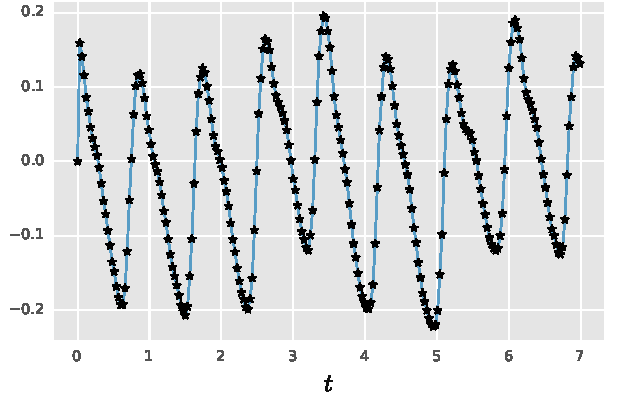
\includegraphics{img/harmonic_trajectory}%
	\caption{%
	A short sequence of the ECG data. %
   	}
	\label{fig:ecg_data}
 \end{figure}
 
 \begin{figure}[htb]%
    \centering%
    \makebox[\textwidth]{%
    \begin{subfigure}[t]{0.5\textwidth+0.4in}%
    	\caption{EM}
    	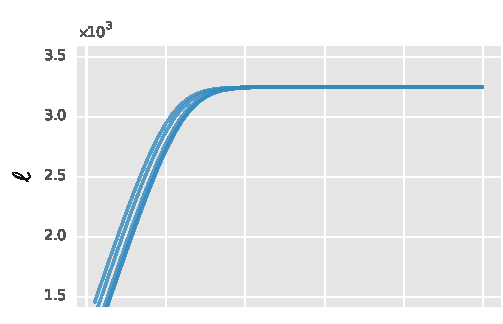
\includegraphics{img/harmonic_em_lh}%
    	%\caption{Convergence of the likelihood with EM}%
		%\label{fig:harmonic_lh_em}%
    \end{subfigure}%
    \begin{subfigure}[t]{0.5\textwidth+0.4in}%
		\caption{BFGS}
		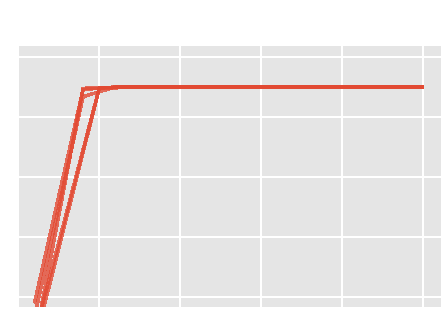
\includegraphics{img/harmonic_bf_lh}%
    	%\caption{Convergence of the likelihood with BFGS}%
		%\label{fig:harmonic_lh_bf}%
    \end{subfigure}}\\%
    \makebox[\textwidth]{%
    \begin{subfigure}[t]{0.5\textwidth+0.4in}%
    	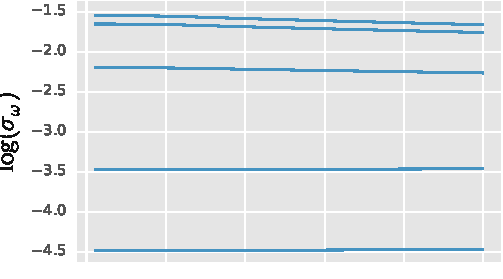
\includegraphics{img/harmonic_em_lqw}%
    	%\caption{Convergence of the likelihood with EM}%
		%\label{fig:harmonic_lh_em}%
    \end{subfigure}%
    \begin{subfigure}[t]{0.5\textwidth+0.4in}%
		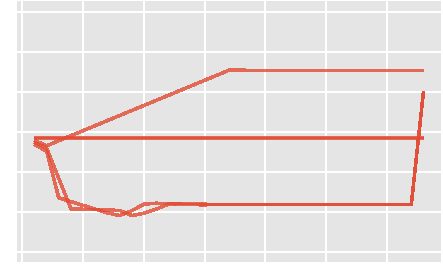
\includegraphics{img/harmonic_bf_lqw}%
    	%\caption{Convergence of the likelihood with BFGS}%
		%\label{fig:harmonic_lh_bf}%
    \end{subfigure}}\\%
    \makebox[\textwidth]{%
    \begin{subfigure}[t]{0.5\textwidth+0.4in}%
    	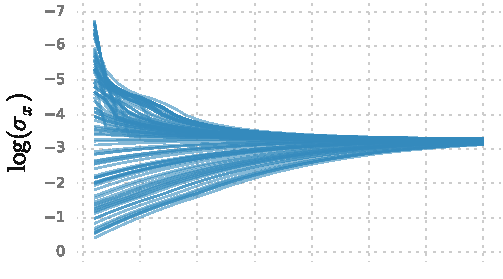
\includegraphics{img/harmonic_em_lqx}%
    	%\caption{Convergence of the likelihood with EM}%
		%\label{fig:harmonic_lh_em}%
    \end{subfigure}%
    \begin{subfigure}[t]{0.5\textwidth+0.4in}%
		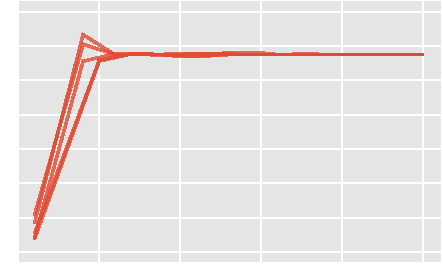
\includegraphics{img/harmonic_bf_lqx}%
    	%\caption{Convergence of the likelihood with BFGS}%
		%\label{fig:harmonic_lh_bf}%
    \end{subfigure}}%\\%
%     \makebox[\textwidth]{%
% 	\begin{subfigure}[b]{0.5\textwidth+0.4in}%
%     	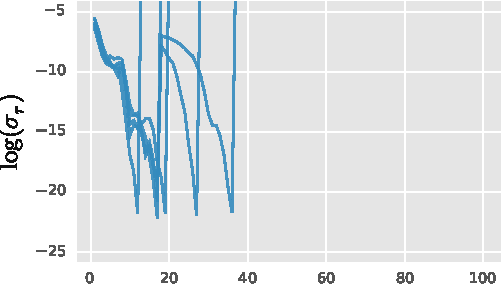
\includegraphics{img/harmonic_em_lr}%
%     	%\caption{Convergence of the likelihood with EM}%
% 		%\label{fig:harmonic_lh_em}%
%     \end{subfigure}%
%     \begin{subfigure}[b]{0.5\textwidth+0.4in}%
% 		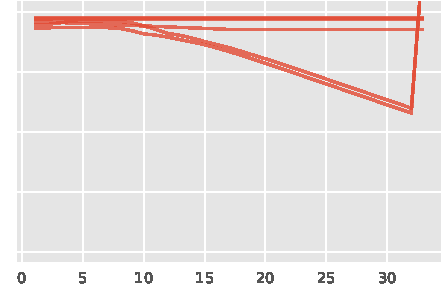
\includegraphics{img/harmonic_bf_lr}%
%     	%\caption{Convergence of the likelihood with BFGS}%
% 		%\label{fig:harmonic_lh_bf}%
%     \end{subfigure}}%
    \caption{Convergence of the likelihood and estimates with EM and BFGS}\label{fig:harmonic_est}
 \end{figure}